\section{Biplots for contingency tables}\label{sec:biplot}
\ixon{biplot}
Like \CA, the biplot
\citep{BraduGabriel:78,Gabriel:71,Gabriel:80,Gabriel:81}
is a visualization method
which uses the SVD to display a matrix in a low-dimensional
(usually 2-dimensional) space.
They differ in the relationships in the data which are portrayed,
however.
In \CA\ the \emph{distances} between row points and
distances between column points are designed to reflect \emph{differences} between the row profiles
and column profiles.
In the biplot, on the other hand,
row and column points are represented by vectors from the origin
such that the projection 
(inner product) of the vector $\vec{a}_i$ for row $i$
on $\vec{b}_j$ for column $j$ approximates the data element
$y_{ij}$,
\begin{equation}\label{eq:biplot1}
 \mat{Y} \approx \mat{A} \mat{B}\trans \iff
 y_{ij} \approx \vec{a}_i \trans \vec{b}_j
 \period
\end{equation}
Geometrically, \eqref{eq:biplot1} may be described as approximating the data value
$\vec{b}_j$ by the projection of the end point of vector $\vec{a}_i$
on $\vec{b}_j$ (and vice-versa).

For quantitative data \citet{BraduGabriel:78} show how the biplot can be used
to diagnose additive relations among rows and columns. For example, when
a two-way table is well-described by a two-factor ANOVA model with no
interaction,
\begin{equation*}%\label{eq:twoway}
y_{ij} = \mu + \alpha_i + \beta_j + \epsilon_{ij}
\end{equation*}
then, the row points, $\vec{a}_i$, and the column points, $\vec{b}_j$,
will fall on two straight lines at right angles to each other in the
biplot.
For a contingency table, the multiplicative relations among
frequencies under independence become additive relations
in terms of log frequency,
and \citet{Gabriel-etal:97} illustrate how biplots of log frequency
can be used to explore associations in two-way and three-way tables.

Several other biplot representations for contingency tables
are described by \citet{Gabriel:95a,Gabriel:95b}, and in a wider
context by \citet{GowerHand:96}.
\citet{Greenacre:93} discusses the relations between biplots and
both CA and MCA, and shows some conditions under which a
\CA\ plot may be interpreted as a biplot.
More general models, with relations to both CA and biplots are
discussed by \citet{Goodman:86,Goodman:91}.

\subsection{Biplots for two-way tables}\label{sec:biplot2}
\ixon{biplot!two-way tables}
For a two-way table, independence
implies that ratios of frequencies should be proportional for any
two rows, $i, i^{\prime}$ and any two columns, $j, j^{\prime}$.
\begin{equation*}
A \perp B \iff \frac{n_{ij}}{n_{i^{\prime} j}} = \frac{n_{ij^{\prime}}}{n_{i^{\prime} j^{\prime}}}
\end{equation*}
Equivalently, the log odds ratio for all such sets of cells should
be zero:
\begin{equation*}
A \perp B \iff \log \theta_{i i^{\prime}, j j^{\prime}} = \log \left( \frac{n_{ij} n_{i^{\prime} j^{\prime}}} {n_{i^{\prime} j}  n_{ij^{\prime}}} \right) = 0
\end{equation*}
Now, if the log frequencies have been
centered by subtracting the grand mean,
\citet{Gabriel-etal:97} show that $\log \theta_{i i^{\prime}, j j^{\prime}}$
is approximated in the biplot (of $\log(n_{ij}) - \overline{ \log(n_{ij}) }$)
\begin{equation*}
\log \theta_{i i^{\prime}, j j^{\prime}} \approx
\vec{a}_i \trans \vec{b}_j - \vec{a}_{i^{\prime}} \trans \vec{b}_j -
\vec{a}_i \trans \vec{b}_{j^{\prime}} + \vec{a}_i \trans \vec{b}_{j^{\prime}}
= ( \vec{a}_i - \vec{a}_{i^{\prime}} )\trans ( \vec{b}_i - \vec{b}_{i^{\prime}} )
\end{equation*}

Therefore, the biplot criterion for independence in a two-way table
is whether \(  ( \vec{a}_i - \vec{a}_{i^{\prime}} )\trans ( \vec{b}_i - \vec{b}_{i^{\prime}} ) \approx 0\) for all pairs of rows, $i, i^{\prime}$,
and all pairs of columns, $j, j^{\prime}$.
But \( ( \vec{a}_i - \vec{a}_{i^{\prime}} ) \) is the vector connecting
$\vec{a}_i$ to $\vec{a}_{i^{\prime}}$ and
 \( ( \vec{b}_j - \vec{b}_{j^{\prime}} ) \) is the vector connecting
$\vec{b}_j$ to $\vec{b}_{j^{\prime}}$, as shown in \figref{fig:bidemo},
and the inner product of any two vectors equals zero \emph{iff} they
are orthogonal.
Hence, this criterion implies that all
lines connecting pairs of row points are orthogonal to lines connecting
pairs of column points, as illustrated in the figure.
\begin{figure}[htb]
  \centering
  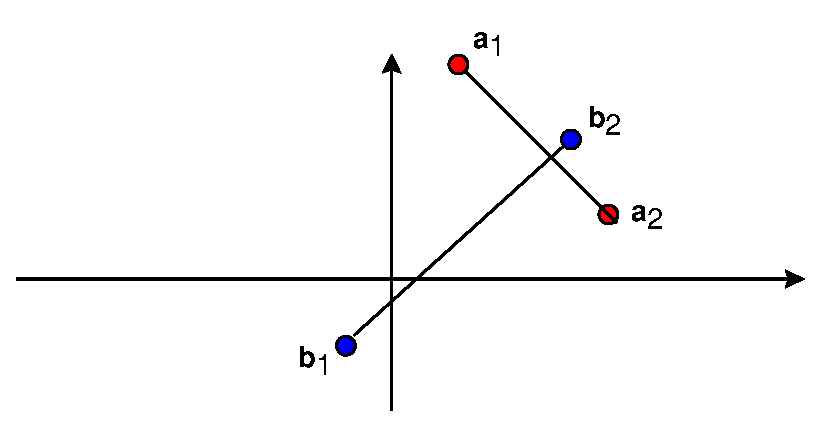
\includegraphics[scale=1]{ch5/fig/bidemo}
  \caption[Independence implies orthogonal vector differences in a biplot of log frequency]{Independence implies orthogonal vector differences in a biplot of log frequency.  The line joining $\vec{a}_1$ to $\vec{a}_2$ represents
 $(\vec{a}_1 - \vec{a}_2)$.  This line is perpendicular to the line
 $(\vec{b}_1 - \vec{b}_2)$ under independence.}  \label{fig:bidemo}
\end{figure}

Thus, when the entire table exhibits independence, the row points
and column points will lie close to two perpendicular lines.
Moreover, a 2-dimensional biplot will account for nearly all of
the variance of the centered log frequencies.
When only a subset of the rows and/or columns are independent,
the points corresponding to those rows and columns will still
lie in orthogonal subspaces, which will be lines or planes
depending on whether a 2D or 3D biplot provides an adequate fit.
An advantage of this method is that it provides a visual indication
of the subsets of rows and columns for which independence does
and does not hold.

\begin{Example}[soccer3]{UK Soccer scores}
We examined the data on UK Soccer scores in \exref{ex:soccer2}
and saw that the number of goals scored by the home and away teams
were largely independent (cf. \figref{fig:soccer2}).
This \Dset\ provides a good test of the ability of the biplot
to diagnose independence.

The biplot analysis is carried out with an enhanced version of
the \macro{BIPLOT} presented in \SSSGref{8,7, A1.2}.
The enhanced version, described in \macref{mac:biplot},
provides automatic equating of the axes
and labeled plots with a variety of interpolation options.

The statements below read the \Dset\ \pname{SOCCER}
and call the \macro{BIPLOT}.  The \mparm{POWER=0}{BIPLOT}
specifies a $\log_{10}$ transformation of the frequencies
contained in the input variables \texttt{A0-A4}.
By default, the \macro{BIPLOT} always standardizes the data
(after transformation, if any) by removing the grand mean,
so the \mparm{STD=NONE}{BIPLOT} indicates no further standardization
is required.
%% input: /users/faculty/friendly/sasuser/catdata/soccer3.sas
%% last modified: 05-Aug-98  9:30
\begin{listing}
title 'UK Soccer scores: Biplot';
data soccer;
   input home $ a0-a4;
datalines;
H0   27 29 10  8  2
H1   59 53 14 12  4
H2   28 32 14 12  4
H3   19 14  7  4  1
H4    7  8 10  2  0
;

%biplot(data=soccer, var=_num_, id=home,
   std=none, power=0,
   out=biplot, anno=bianno,
   symbols=circle dot, interp=none);
\end{listing}


By default, the macro produces a plot of the first two biplot dimensions.
As with the \macro{CORRESP}, the axes are equated in this plot
by default (when the \pname{HAXIS} and \pname{VAXIS} parameters are
not specified).  Sometimes, you may wish
to inspect an initial plot and then
rescale it, as illustrated in \exref{ex:haireye3} and \exref{ex:mental1}.
The macro also produces an \ODS\ of coordinates (\mparm{OUT=BIPLOT}{BIPLOT}) and an \ADS\ (\mparm{ANNO=BIANNO}{BIPLOT}) containing category labels,
which may be used for further customization.

The default plot showed that all of the category points, except for A2 and H2, fell along
separate orthogonal straight lines parallel to the coordinate axes.
The two biplot dimensions account for 99.8\% of the variance.
The statements below are used to find the locations of these lines
from the means of the \pname{DIM1} and \pname{DIM2} coordinates
and append Annotate instructions to draw them to the \pname{BIANNO} \ADS.
The \PROC{GPLOT} step produces \figref{fig:soccer3}.
\begin{figure}[htb]
  \centering
  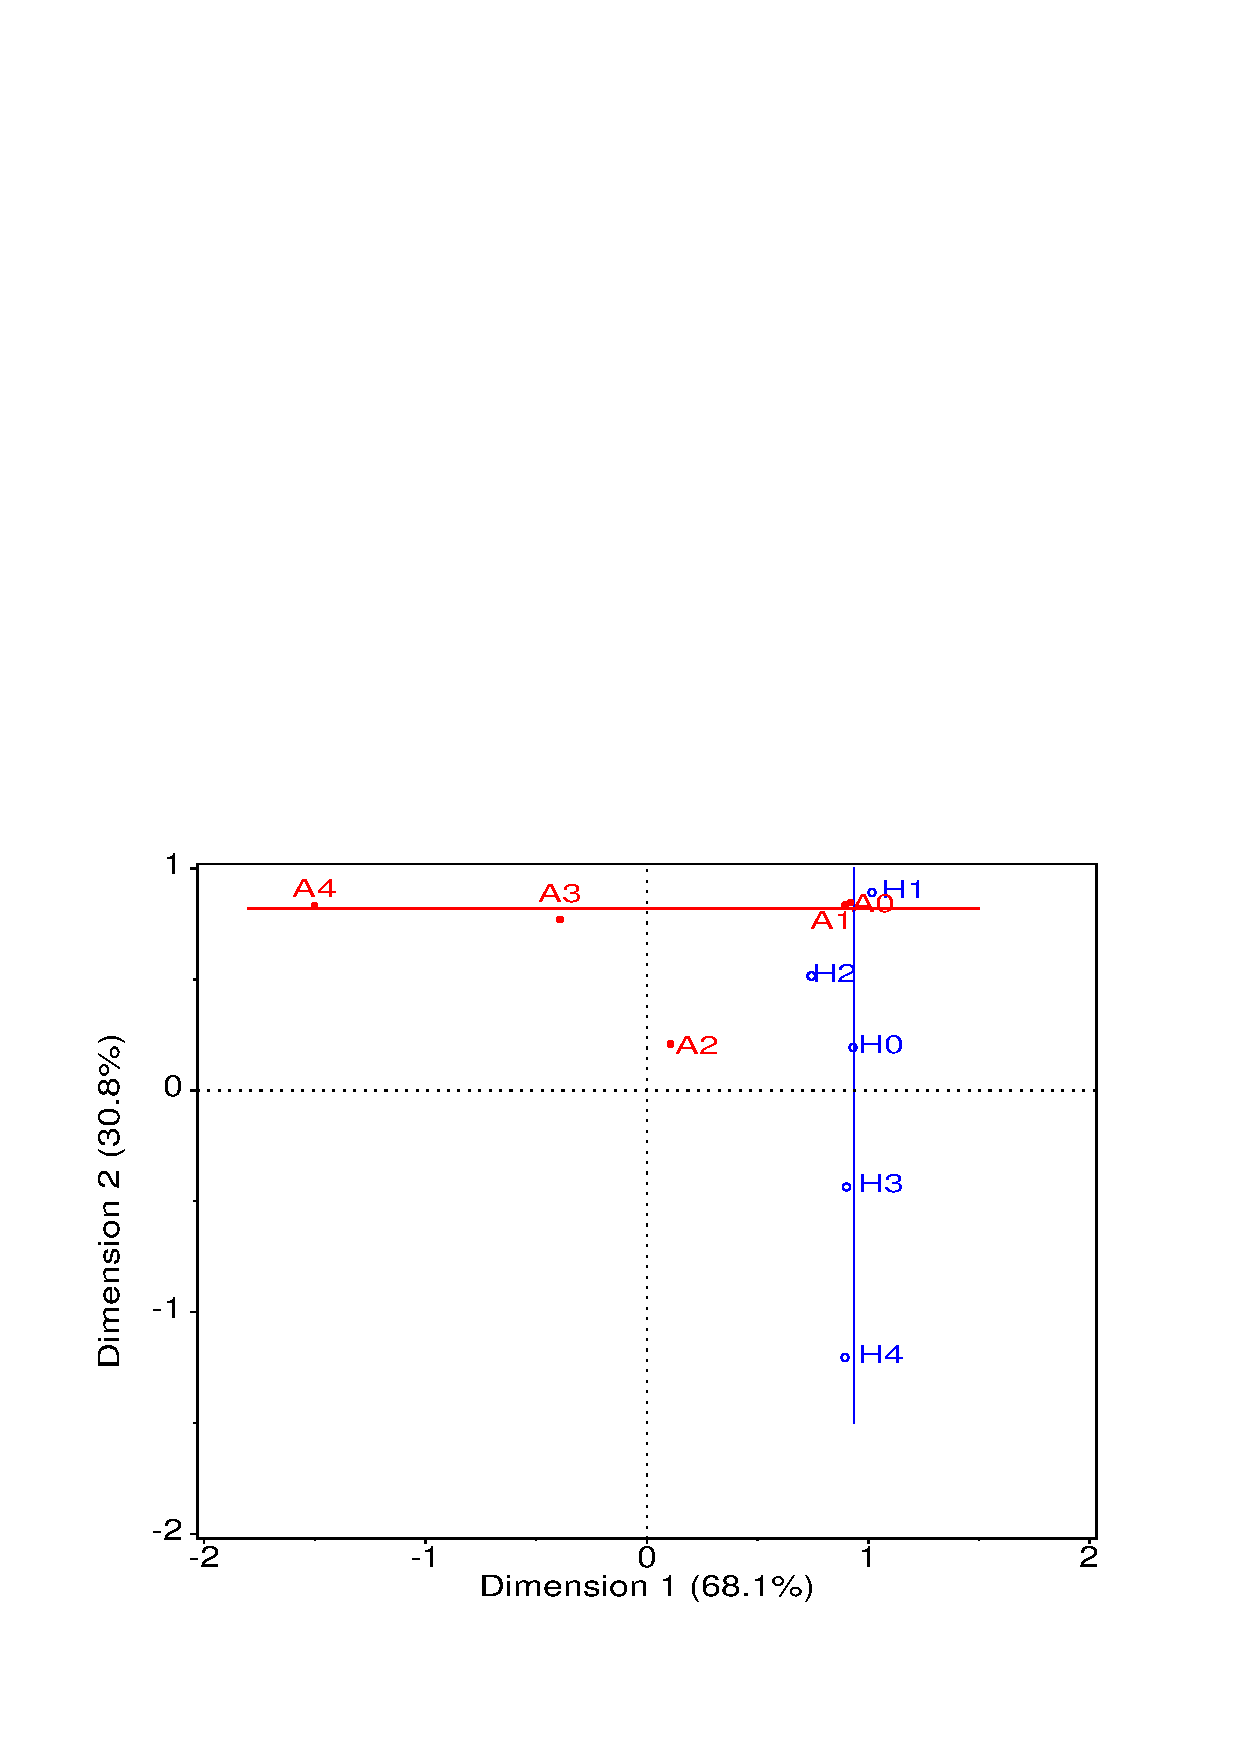
\includegraphics[scale=.6]{ch5/fig/soccer3}
  \caption[Biplot of UK Soccer scores]{Biplot of UK Soccer scores.
  Independence is shown when the row and column points lie on orthogonal
  lines.}  \label{fig:soccer3}
\end{figure}
%% input: /users/faculty/friendly/sasuser/catdata/soccer3.sas
%% last modified: 05-Aug-98  9:30
\begin{listing}
*-- Find mean coordinates (except A2, H2);
proc means data=biplot noprint;
   where (_name_ not in ('A2', 'H2'));
   var dim1 dim2;
   by _type_;
   output out=means mean=;

*-- Draw lines passing thru the means, parallel to axes;
data lines;
   set means;
   xsys='2'; ysys='2';
   length function color $8;
   if _type_ = 'OBS' then do;
      x = dim1; color='blue';
      y = -1.5; function='move';  output;
      y = +1.0; function='draw';  output;
      end;
   else do;
      y = dim2; color='red';
      x = -1.8; function='move';  output;
      x = +1.5; function='draw';  output;
      end;

*-- Append to annotate data set;
data bianno;
   set bianno lines;

title;
proc gplot data=biplot;
   plot dim2 * dim1 = _type_ /
         anno=bianno frame nolegend
         href=0 vref=0 lvref=34 lhref=34
         vaxis=axis1 haxis=axis2
         vminor=1 hminor=1
         name="soccer3" des="Biplot of log(freq)";
      axis1 order=(-2 to 1) length=4.5in label=(a=90) ;
      axis2 order=(-2 to 2) length=6in;
      symbol1 v=circle c=blue i=none;
      symbol2 v=dot    c=red  i=none;
   run;
\end{listing}

We see that all the A points (except for A2) and all the H points (except for H2) lie along straight lines, and these lines are indeed at right angles,
signifying independence.
The fact that these straight lines are parallel to the coordinate axes is
incidental, and unrelated to the independence interpretation.
\end{Example}
\ixoff{biplot!two-way tables}

\subsection{Biplots for three-way tables}
\ixon{biplot!three-way tables}
Biplot displays for three-way tables may be constructed by means of the
``stacking'' approach used in \CA\ described in \secref{sec:ca-multiway}.
That is, a
three-way table,  \(I \times  J \times  K\),
can be represented (in several ways) as a two-way table, with two
variables combined interactively.

As before, consider a three-way $ABC$ table structured as
\(I J \times  K\) so that variables $A$ and $B$ define the rows and
variable $C$ defines the columns.
(Equivalent results obtain for any permutation of the variables.)
Then, a biplot will have row points, $\vec{a}_{ij}$ and column points
$\vec{b}_{k}$ which approximate
\begin{equation*}
\log ( n_{[ij]k} ) - \overline{ \log ( n_{[ij]k} ) }
 \approx \vec{a}_{ij}\trans \vec{b}_{k}
\end{equation*}

By the same arguments of \secref{sec:biplot2},
when $\{A, B\} \perp C$, that is, when the model of joint independence,
$[A B][C]$ holds, then the $\vec{a}_{ij}$ row points will fall on
one straight line and the $\vec{b}_{k}$ will fall on another line,
perpendicular to the first.

Other configurations of points along lines serve as tests for other
models of independence.
For example, if, for a given level $j^{\star}$ of variable $B$, the
points $\vec{a}_{ij^{\star}}$ are collinear and orthogonal
to the line formed by the $\vec{b}_{k}$ of variable $C$,
then \emph{partial independence},
$A \perp C \given B_{j^{\star}}$ holds for level $j^{\star}$.
If this is true for all levels of variable $B$,
then $A$ is conditionally independent of $C$, given $B$,
$\{ A \perp C \} \given B$, or the \loglin\ model $[A B][C B]$.
Thus, for conditional (respectively, partial) independence, the
$\vec{a}_{ij^{\star}}$ points fall on \emph{separate} straight lines
orthogonal to the $\vec{b}_{k}$ for all (respectively, some) levels
of variable $B$, while for joint independence, they all fall on the
\emph{same} straight line.
\ix{biplot!partial independence}
\ix{biplot!conditional independence}
\ix{partial independence!biplot}
\ix{conditional independence!biplot}

Hence, for suitable rearrangement of the variables into a three-way
table, the biplot can be used to identify the major models of
independence.

\begin{Example}[employ2]{Employment status data}
\exref{ex:employ} examined questions of partial and conditional independence
in the Danish employment status data.
We saw (cf. \figref{fig:employp}) that whether a worker was re-employed ($E$)
was independent of length ($L$) of previous employment for those workers
laid off due to closure, but re-employment was strongly associated
for workers who were replaced.

\begin{figure}[htb]
  \centering
  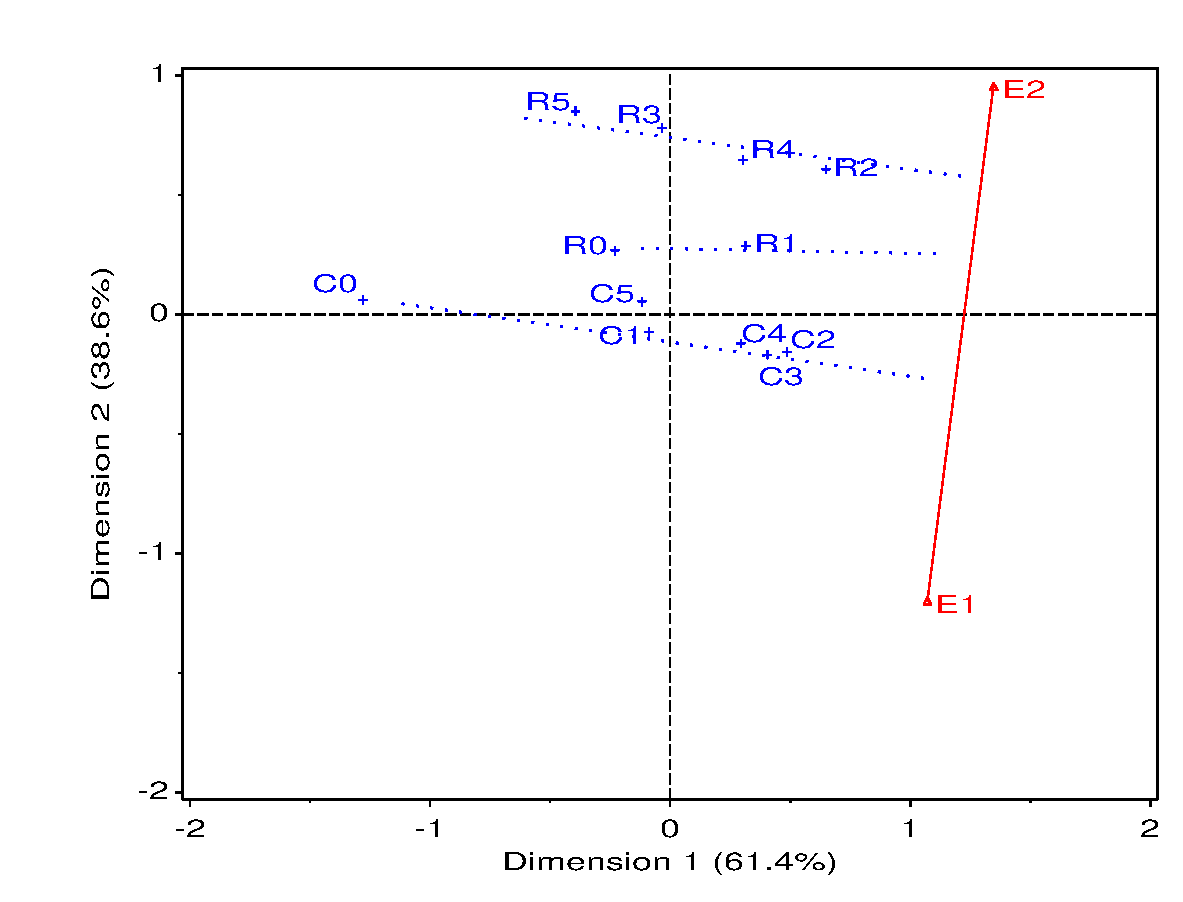
\includegraphics[scale=.8]{ch5/fig/employe}
  \caption[Biplot for Employment status data]{Biplot for Employment status data}  \label{fig:employe}
\end{figure}

The statements below read the data (see \tabref{tab:employ}) in frequency form
and reshape the \pname{COUNT} variable as a $12 \times 2$ matrix
with the variables \pname{CAUSE} and \pname{LENGTH} defining the rows
and the two levels of \pname{EMPLOYED} as columns.
The levels of length of previous employment are identified by the
digits 0 to 6, and the levels of \pname{CAUSE} by `C' (closure) and
`R' (replacement),
which are combined in the \pname{ID} variable for the matrix rows.
The column variables \pname{E1} and \pname{E2} are the two levels
of employment in sorted order, `No' and `Yes'.
%% input: /users/faculty/friendly/sasuser/catdata/employ.sas
%% last modified: 06-Aug-98 11:53
\begin{listing}
data employ;
   input length $ @;
   do cause ='Close  ', 'Replace';
      do employed = 'Yes', 'No';
         input count @;
         output;
         end;
      end;
   input;
datalines;
 0     8   10     40   24 
 1    35   42     85   42 
 2    70   86    181   41 
 3    62   80     85   16 
 4    56   67    118   27 
 5    38   35     56   10 
;
*-- Reshape as two column matrix ([CL][E]);
proc sort data=employ;
   by cause length employed ;
proc transpose prefix=e out=employ2;
   var count;
   by cause length;
data employ2;
   set employ2;
   drop _name_;
   id = substr(cause,1,1) || length;

axis1 order=(-2 to 1) length=4.875in
   label=(a=90);
axis2 order=(-2 to 2) length=6.5in;
%biplot(data=employ2, id=id, var=e1 e2,
   std=none, power=0,
   out=biplot, anno=bianno, vaxis=axis1, haxis=axis2,
   symbols=plus triangle, interp=none join);
\end{listing}

The call to the \macro{BIPLOT} produces the graph shown in \figref{fig:employe}.
The line joining E1 and E3 was produced by the \mparm{INTERP=NONE JOIN}{BIPLOT}.
The dotted lines were drawn manually (and therefore approximately) in the Graphics Editor.

We see that the points for closure lie approximately along a line perpendicular to the line for E1-E2, indicating partial independence
of employment status
and length for the closure workers (points C0-C5).
The R points for replaced workers do not all fall on one line,
so there is no overall partial independence for these workers;
however, for those workers previously employed for 3 months or more
(R2-R5),  the points are nearly collinear and orthogonal to E1-E2.
\ixoff{biplot!three-way tables}
\ixoff{biplot}
\end{Example}
